    \begin{figure}[h]
    \centering
    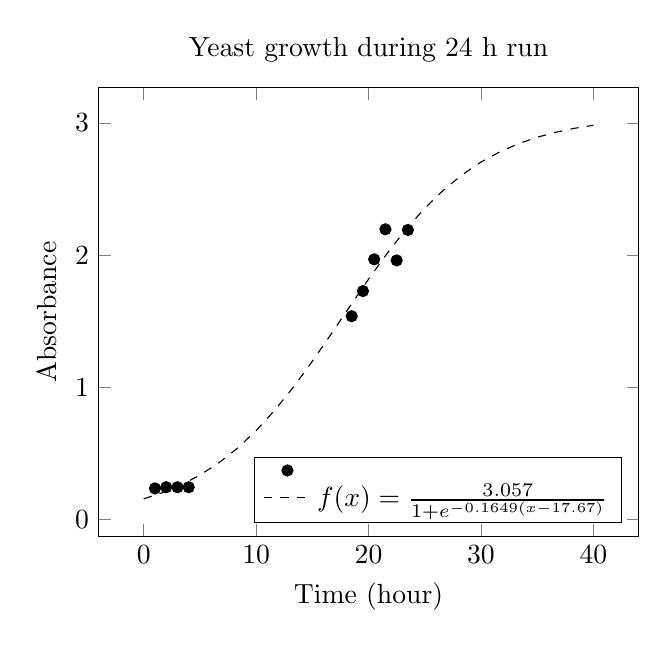
\begin{tikzpicture}[]
        \begin{axis}[title={Yeast growth during 24 h run}, ylabel=Absorbance , xlabel=Time (hour), legend pos = south east, domain=0:40]
            \addplot[only marks] table{
                1	0.236
                2	0.245
                3	0.245
                4	0.245
                18.5	1.538
                19.5	1.728
                20.5	1.968
                21.5	2.195
                22.5	1.96
                23.5	2.19
            };
            \addplot[dashed]{ 3.05695/(1+e^(-0.164931*(x-17.6678)) )};
        \addlegendentry{}
        \addlegendentry{$f(x) = \frac{3.057}{1+e^{-0.1649(x-17.67)}}$}   
        \end{axis}
    \end{tikzpicture}
    \end{figure}